
\section{Item Association}

\label{sec:item}

Items are the most essential nodes in any e-commerce knowledge graph, since the ultimate goal of e-commerce platform is to make sure that customers can easily find items that satisfy their needs.
So far, we conceptualize user needs as e-commerce concepts and interpret
them using the structured primitive concepts.
The last thing is to associate billions of items in Alibaba with all the concepts (both primitive and e-commerce) to form the complete AliCoCo.

Since primitive concepts are similar to single-value tags and properties, 
the mapping between primitive concepts and items are relatively straightforward.
Therefore, in this section, we mainly introduce the methodology of associating items with e-commerce concepts, where the latter ones representing certain shopping scenarios usually carry much more complicated semantic meanings.
Besides, the association between an e-commerce concept and certain items can not be directly inferred from the association between corresponding primitive concepts and their related items due to a phenomenon called ``semantic drift''.
For example, charcoals are necessary when we want to hold an ``outdoor barbecue'',
however, they have nothing to do with primitive concept ``\textit{Location: Outdoor}''.

\begin{figure}[th]
	\centering
	\epsfig{file=figures/matching.eps, width=1\columnwidth}
	\caption{Overview of knowledge-aware deep semantic matching model for association between e-commerce concepts and items.
	}
	\label{fig:matching}
\end{figure}

We formulate this task as \textit{semantic matching} between texts \cite{huang2013learning,pang2016text,yang2019simple}, since we only use textual features of items at current stage. 
The main challenge to associate e-commerce concepts with related items is that the length of the concept is too short so that limited information can be used.
Due to the same reason, there is a high risk that some of less important words may misguide the matching procedure.
To tackle it, we propose a knowledge-aware deep semantic matching model shown in \figref{fig:matching}.
The inputs are a sequence of concept words and a sequence of words from the title of a candidate item.
We obtain input embeddings concatenating pre-trained word embeddings of two sequences with their POS tag embedding and NER tag embedding (similar to \secref{sec:tagging}):
$\{\bi{w}_1, \bi{w}_2,...\bi{w}_m\}$
and 
$\{\bi{t}_1, \bi{t}_2,...\bi{t}_l\}$.
we adopt wide CNNs with window size $k$ to encode the concept and item respectively:
\begin{equation}
\bi{w'}_i = \cnn([\bi{w}_{i-k/2}, ..., \bi{w}_i, ..., \bi{w}_{i+k/2}])
\end{equation}
%\begin{equation}
%\bi{w'} = \maxpool([..., \bi{w'}_i, ...]) 
%\end{equation}
\begin{equation}
\bi{t'}_i = \cnn([\bi{t}_{i-k/2}, ..., \bi{t}_i, ..., \bi{t}_{i+k/2}])
\end{equation}
%\begin{equation}
%\bi{t'} = \maxpool([..., \bi{t'}_i, ...]) 
%\end{equation}
Intuitively, different words in the concept should share different weights when matching to the item, and vice versa.
Therefore, we apply attention mechanism \cite{bahdanau2014neural,luong2015effective} in our model.
An attention matrix is used to model the two-way interactions simultaneously. 
The values of attention matrix are defined as below:
\begin{equation}
att_{i,j} = \bi{v}^T\tanh(\bi{W}_1\bi{w'}_i+\bi{W}_2\bi{t'}_j)
\end{equation}
where $i \in [1, m]$ and $j \in [1, l]$, $\bi{v}$, $\bi{W}_1$ and $\bi{W}_1$ are parameters.
Then the weight of each concept word $w_i$ and title word $t_i$ can be calculated as:
\begin{equation}
	\alpha_{wi} = \frac{exp(\sum_{j}att_{i,j})}{\sum_{i}exp(\sum_{j}att_{i,j})}
\end{equation}
\begin{equation}
\alpha_{tj} = \frac{exp(\sum_{i}att_{i,j})}{\sum_{j}exp(\sum_{i}att_{i,j})}
\end{equation}
Then, we obtain concept embedding \bi{c} as:
\begin{equation}
	\bi{c} = \sum_{i}\alpha_{wi}\bi{w'}_i
\end{equation}
and item embedding \bi{i} similarly.

To introduce more informative knowledge to help semantic matching,
we obtain the same knowledge embedding sequence in \secref{sec:classification}:
\begin{equation}
	\bi{k}_i = \docvec(Gloss(w_i))
\end{equation}
Besides, we obtain class label id embedding $\bi{cls}_j$
of $j$th primitive concept linked with current e-commerce concept.
Thus, there are three sequences on the side of concept:
\begin{eqnarray*}
& \{\bi{kw}_i\} = \{\bi{kw}_1,\bi{kw}_2,...\bi{kw}_{2*m+m'}\} = \\
& \{\bi{w}_1,\bi{w}_2,...\bi{w}_m,\bi{k}_1,\bi{k}_2,...\bi{k}_m,\bi{cls}_1,\bi{cls}_2,...\bi{cls}_{m'}\}
\end{eqnarray*}
where $m'$ is the number of primitive concepts.
In the side of item, we directly use the sequence of word embedding $\{\bi{t}_i\} = \{\bi{t}_1, \bi{t}_2,...\bi{t}_l\}$.
Then, we adopt the idea of Matching Pyramid \cite{pang2016text}, 
the values of matching matrix in $k$th layer are defined as below:
\begin{equation}
	match_{i,j}^k = \bi{kw}_i^{T}\bi{W}_k\bi{t}_j
\end{equation}
where $i \in [1, 2*m+m']$ and $j \in [1, l]$.
Each layer of matching matrix are then fed to 2-layer of CNNs and max-pooling operation to get a matching embedding $\bi{ci}^k$.
The final embedding of matching pyramid $\bi{ci}$ is obtained by:
\begin{equation}
\bi{ci} = \mlp([;\bi{ci}^k;])
\end{equation}

The final score measuring the probability is calculated as:
\begin{equation}
	score = \mlp([\bi{c};\bi{i};\bi{ci}])
\end{equation}



%The relevance computation between concepts and items require extremely high precision since one bad case could harm user experience badly, and high recall, otherwise some items will not be found through certain concepts forever.
%The challenge here is that concept is a term-based phrase with some attributes and item is a complex structure containing various information such as title, figure, attributes, description or even a short video.
%Matching these two heterogeneous contents with high recall and precision is not a simple task.




